\begin{frame}
    \frametitle{Objetivos}
    \begin{itemize}
        \item O objetivo deste módulo é permitir perceber qual o conjunto de
        ações que devem ser despoletadas de modo a configurar um equipamento com
        um determinado contexto.
    \end{itemize}    
    \begin{figure}
        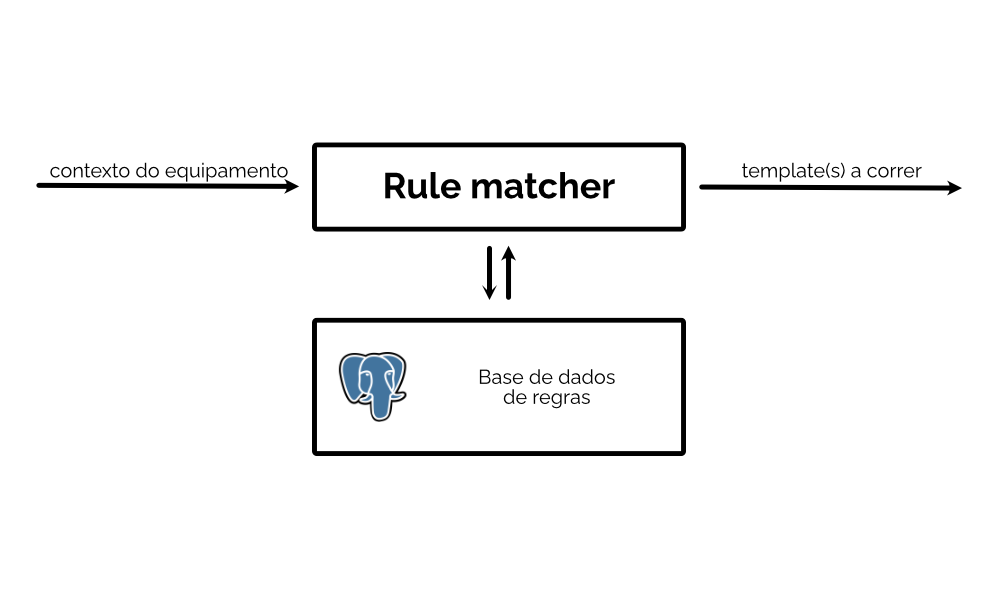
\includegraphics[width=0.7\textwidth]{./assets/rule_matcher/rule_matcher.png}
    \end{figure}
\end{frame}

\begin{frame}
    \frametitle{Conceito de \textit{regra} e definição}
    \begin{table}
        \centering
        \begin{tabular}{ |c|c|c| }
          \hline
          \textbf{Parâmetro} & \textbf{Tipo de dados} & \textbf{Caráter} \\ \hline
          token & inteiro & metadado \\ \hline
          firmwareVersion & string & parâmetro \\ \hline
          ipAddress & string & parâmetro \\ \hline
          olt & string & parâmetro \\ \hline
          card & string & parâmetro \\ \hline
          interface & string & parâmetro \\ \hline
          equipmentId & string & parâmetro \\ \hline
          password & string & parâmetro \\ \hline
          vendor & string & parâmetro \\ \hline
          parameters & array & parâmetro \\ \hline
          priority & integer & metadado \\ \hline
          template & string & metadado \\ \hline
        \end{tabular}
        \caption{Parâmetros que integram as regras}
      \end{table}
\end{frame}
